\newpage
\chapter*{Simulations}
\addcontentsline{toc}{chapter}{Simulations} 




% Reconsider later if some if this is better placed in methods section
% or under different title
\section*{Frictional properties of the intact graphene sheet}
The friction measurment simulation is governed by the following parameters, which is divided into three sub categories for the purpose of this thesis as shown in table \ref{tab:param}.



\begin{table}[H]
  \begin{center}
  \caption{Parameters of the numerical procedure for measuring friction.}
  \label{tab:param}
  \begin{tabular}{ | c | m{8cm}| m{5cm}|} 
    \hline
    Category & Parameter name: description & Category purpose \\ 
    \hline
    Physical & 
    \begin{itemize}
      \item[-] T: Temperature for the Langevin thermostat.
      \item[-] $v_{drag}$: Drag speed for the sheet translation.
    \end{itemize} &
    Parameters that we expect to have an inevitably effect on the system friction properties, for which the choice will be a baseline for our studies.
    \\ \hline
    Measurement & 
    \begin{itemize}
      \item[-] $dt$: Integration timestep.
      \item[-] $t_R$: Relaxtion time before strething.
      \item[-] Pauses between stretch and adding normal force and between dragging the sheet.  
      \item[-] Stretch Speed: How fast to stretch the sheet.
      \item[-] $K$: Spring constant for the spring responsible of translating the sheet. An infinte spring constant is achieved by moving the end blocks as a rigid body (Lammps: fix move).
      \item[-] Drag Length: How far to translate the sheet.
      \item[-] Sheet size: Spatial size of the 2D sheet.  
    \end{itemize} &
    Paramters that effects the simulation dynamics and the 'experimental procedure' that we a mimicking. We aim to choose to these paramters such that the friction properties is stable for small perturbations.  \\ \hline
    ML input & 
    \begin{itemize}
      \item[-] Sheet configuration: A binary matrix containing information of which atoms is removed (0) and which is still present (1) in the graphene structure.
      \item[-] Scan angle: The direction for which we translate the sheet.
      \item[-] Stretch amount: The relative sheet stretch in percentage.
      \item[-] $F_N$: Applied normal force to the end blocks.
    \end{itemize} &
    The ramaining paramters that serve as the governing variables in the optimization process for certain friction properties and is thus the input variables for the ML part. 
    \\ \hline
  \end{tabular}
  \end{center}
\end{table}


We should try to set the physcis and measurement parameters in such a way that we reduce computation speed where it is doesn't infer with the frictional properties study.

We need to define some ranges for the ML input paramters. $F_N$, stretch ranges where it is not prone to ruptures. The configuration it self does not have clear rules but is also being regulated by the no rupture requirement. 

\newpage
\subsection{Baseline}

\subsubsection{Single measurement}
\paragraph*{Force oscillations}

We first assess the raw data for the friction force $F_{\parallel}$ parallel to the drag direction as seen in figure \ref{fig:drag_Ff}. The sample rate is 10 ps$^{-1}$ for which we sample the the mean of all previous timesteps. We observe that the data carriers oscillations on different time scales. By applying a savgol filter to data with a polyorder of 5 and window length corresponding to a drag length of 3.0 Å (or time interval 15.0 ps) we can qualitatively point out at least two different frequencies of osccilation. On figure \ref{fig:drag_Ff_10} we see roughly three waves on the savgol filter corresponding to one frequency, while on \ref{fig:drag_Ff_100} the same savgol filter reveals an even slower frequency on top of the first creating a visual patterns of a wavepacket.

\begin{figure}[H]
  \centering
  \begin{subfigure}[b]{0.49\textwidth}
      \centering
      \includegraphics[width=\textwidth]{figures/baseline/drag_Ff_10Å.pdf}
      \caption{Drag length of 10 Å.}
      \label{fig:drag_Ff_10}
  \end{subfigure}
  \hfill
  \begin{subfigure}[b]{0.49\textwidth}
      \centering
      \includegraphics[width=\textwidth]{figures/baseline/drag_Ff_100Å.pdf}
      \caption{Drag length of 100 Å.}
      \label{fig:drag_Ff_100}
  \end{subfigure}
  \hfill
     \caption{Friction force $F_\parallel$ between (full) sheet and substrate with respect to the drag direction vs. drag length. The drag length is measured by the constant movement of the virtual atom and not the COM of the sheet. The red line represents a savgol filter with window polyorder 5 and windoew length 150 (corresponding to a drag length of 3 Å or a time window of 15 ps)}
     \label{fig:drag_Ff}
\end{figure}

By performing a Forward Fourier Transform of the data (using FFT) we can quantitavely idendity some of the leading frequencies as seen in figure \ref{fig:ft_a}. By plotting the two most dominant frequencies $f_1 = 0.0074$ ps $^{-1}$ and $f_2 = 0.0079$ ps $^{-1}$ as $\sin{(2\pi f_1)} + \sin{(2\pi f_2)}$ we find a convincing fit to the observed wavepacket shape as seen in figure \ref{fig:ft_b}. By using the trigonometric identity

\begin{align*}
\sin (\alpha+\beta) &= \sin (\alpha) \cos (\beta) + \cos (\alpha) \sin (\beta), \\
\sin (\alpha-\beta) &= \sin (\alpha) \cos (\beta) - \cos (\alpha) \sin (\beta),
\end{align*}
and decomposing $f_1 = a - b$, $f_2 = a + b$ we can rewrite the sine sum as the sinusoidal product
\begin{align*}
  \sin(2\pi f_1) \sin(2\pi f_2) &= \sin(2\pi (a - b)) \sin(2\pi (a + b)) \\
  &= \sin(a)\cos(b) + \cancel{\cos(2\pi a)\sin(2\pi b)} + \sin(2\pi a)\cos(2\pi b) - \cancel{\cos(2\pi a)\sin(2\pi b)} \\
  &= 2 \sin(2\pi a) \cos(2\pi b),
\end{align*} 

with 
\begin{align*}
  a = \frac{f_1 + f_2}{2} &= 0.0763 \pm 0.0005 \text{ps}^{-1},& 
  b = \frac{f_2 - f_1}{2} &= 0.0028 \pm 0.0005 \text{ps}^{-1},& \\
  &= 0.381 \pm 0.003 \text{Å}^{-1},& 
  &= 0.014 \pm 0.003 \text{Å}^{-1},& 
\end{align*}

where the ladder frequency is denoted with respect to drag length. This makes us recognize the fast osccilation frequency as $a$ and the slower frequency as $b$. We also take note of the longest period in the data $T_b = 1/b \sim 357$ ps $\sim 71$ which will be relevant for the evaluation of measurement incertainty.



\begin{figure}[H]
  \centering
  \begin{subfigure}[b]{0.49\textwidth}
    \centering
    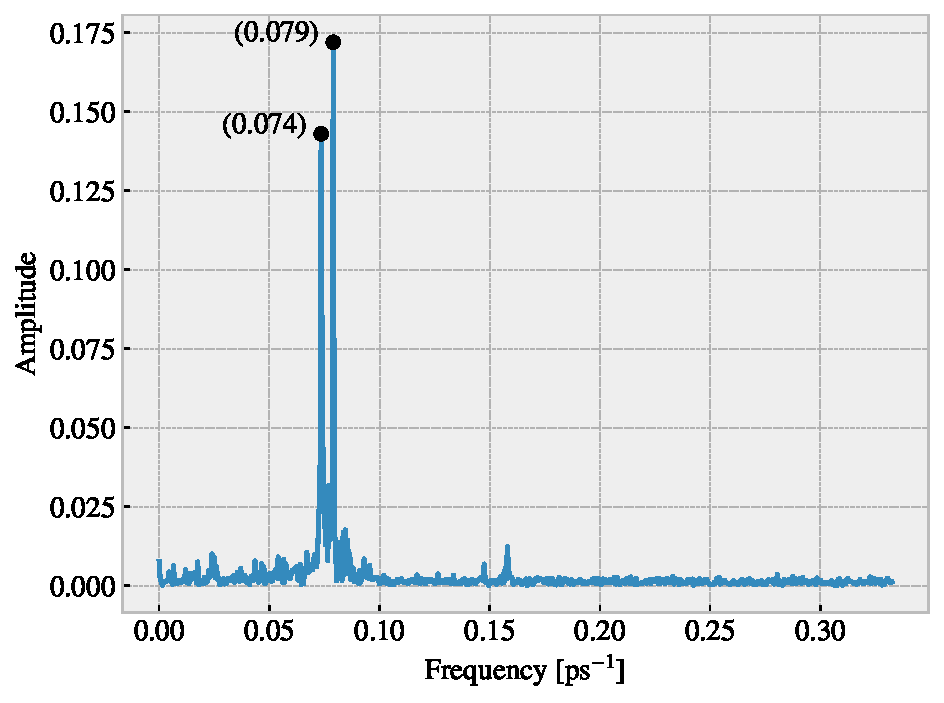
\includegraphics[width=\textwidth]{figures/baseline/ft_zoom.pdf}
    \caption{Reduced frequency range.}
    \label{fig:ft_a}
  \end{subfigure}
  \hfill
  \begin{subfigure}[b]{0.49\textwidth}
      \centering
      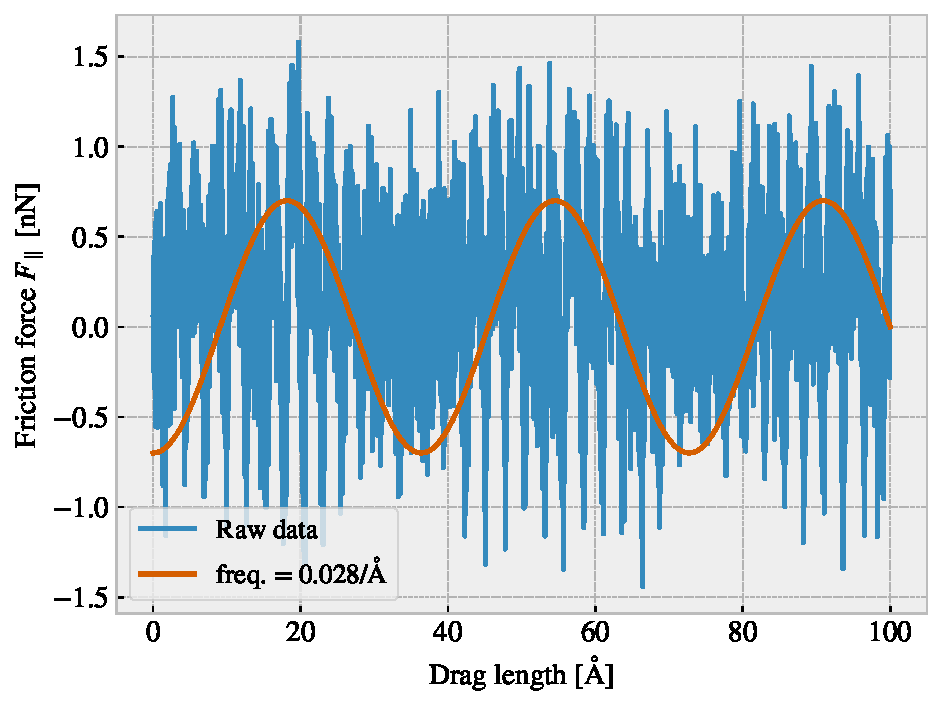
\includegraphics[width=\textwidth]{figures/baseline/ft_sine.pdf}
      \caption{Selected frequencies applied to data from figure \ref{fig:drag_Ff_100}}
      \label{fig:ft_b}
  \end{subfigure}
  \caption{Fourier transform on data shown in figure \ref{fig:drag_Ff}.}
  \label{fig:ft}
\end{figure}


\paragraph*{Decompositions}

In the previous analysis we have looked only as the friction force for the full
sheet, including the pullblocks which is locked off during the drag, and with
respect to the drag direction. \par
Since we are only applying cuts to the inner sheet (excluding the pull blocks),
it might seem more natural to only consider the friction on that part. If the
desired frictional properties can be observed from the inner sheet we can always
scale the relative size between inner sheet and pull block. However, when
looking at the time series of friction force decomposed onto inner sheet and
pull block (figure \ref{fig:decomp_group}) we observe the friction force arrising
from those parts is seemingly antisymmetric. That is, the fricitonal pull on the
substrate is oscillating between the inner sheet and the pullblock. Remembering
that the normal forc eis only applied to the pull block we might take this as an
integrated feature of the system. An interesting nonlinear friction coefficient
might depend on this internal distribution of forces. Hence we hedge our bets an
use the full sheet friction force. \par
Similar we might question the decision of
only considering the frictional force projected on the direction of the drag as
we are neglecting the ``side shift'' induced during the drag phase. In figure \ref{fig:decomp_direc} we see the decomposition into force components parallel $F_{\parallel}$ and perpendicular $F_{\perp}$ to the drag direction respectively. We see that the most dominant trends is projected into the parallel component. If we want to include the perpendicular component as well we would have to evaluate the friction as the length of the vector for which we loose the sign of direction. Hence we would only get positive contributions, meaning a resisting force, which is not faithfully capturing the sheet oscillaitons that make the friction forces act both against in with the direction of drag. By this argument we decide to use only the parallel component going forward. 

\begin{figure}[H]
  \centering
  \begin{subfigure}[b]{0.49\textwidth}
    \centering
    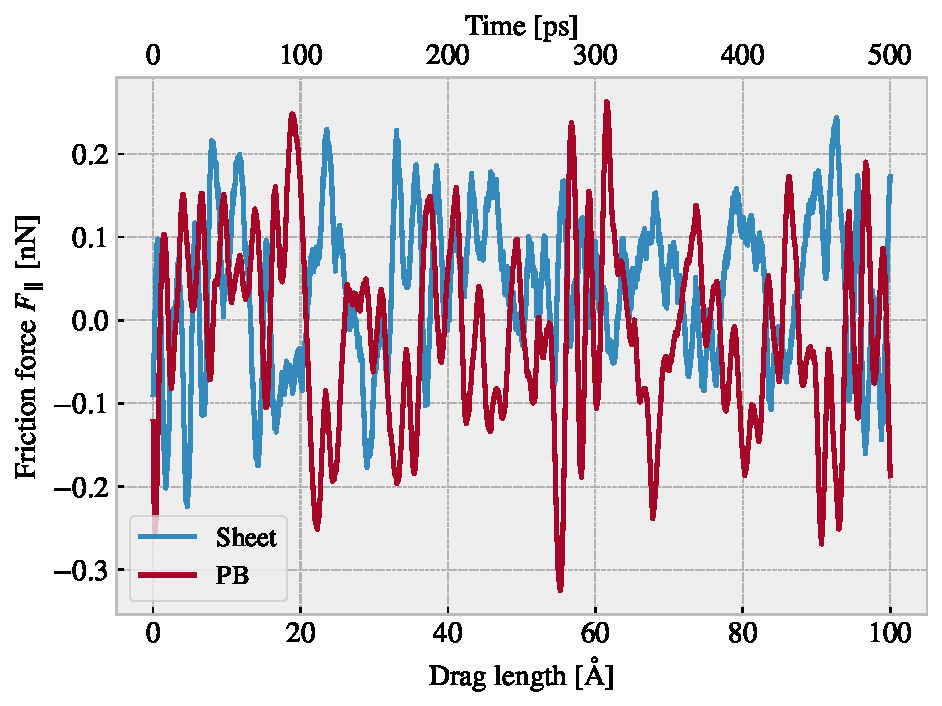
\includegraphics[width=\textwidth]{figures/baseline/decomp_group.pdf}
    \caption{Decomposition into group inner sheet (sheet) and pull blocks (PB).}
    \label{fig:decomp_group}
  \end{subfigure}
  \hfill
  \begin{subfigure}[b]{0.49\textwidth}
      \centering
      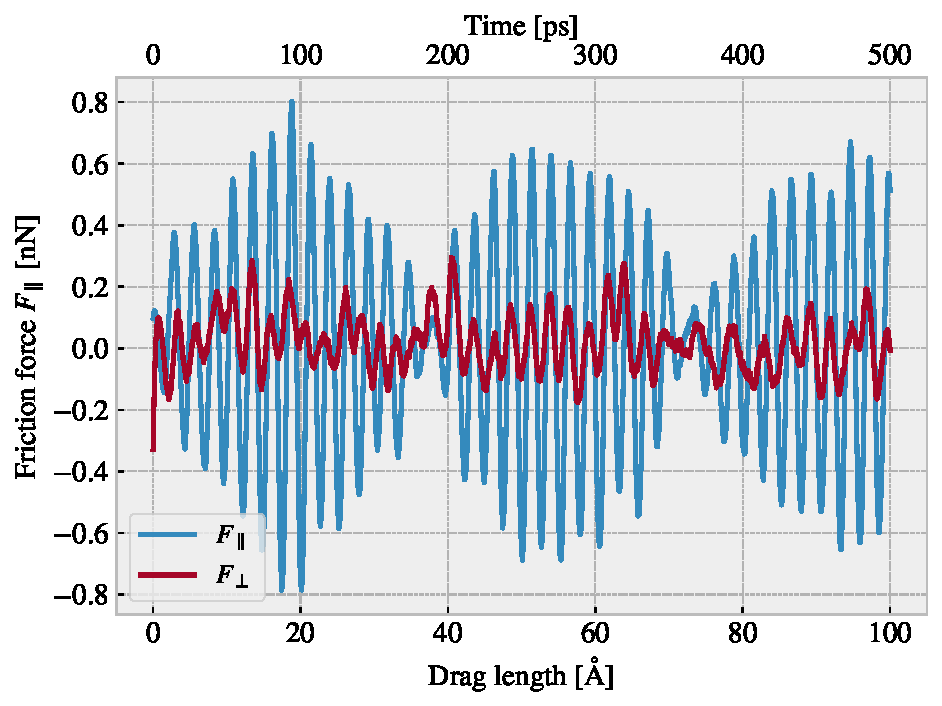
\includegraphics[width=\textwidth]{figures/baseline/decomp_direc.pdf}
      \caption{Decomposition into parallel ($\parallel$) and perpendicular $(\perp)$ to drag direction.}
      \label{fig:decomp_direc}
  \end{subfigure}
  \caption{Decomposition into parallel ($\parallel$) and perpendicular $(\perp)$ to drag direction showing the savgol filter applied}
  \label{fig:decomp}
\end{figure}


\paragraph*{Center of mass path}

From the previous observations we already have evidence of a stick slip behaviour, judging from the friction oscillations in figure \ref{fig:drag_Ff}, and motion partial motion perpendicular to the drag direction, judging from the perpendicular force component in figure \ref{fig:decomp_direc}. By looking at the $x,y$-position for the center of mass (COM) we can see the stick slip motion manifested as a variation in COM speed combinned with a side to side motion as shown in figure $\ref{fig:COM_path_K0}$. To increase this effect we also show the same plot with a spring ... move with spring constant 30 N/m in figure \ref{fig:COM_path_K30}. While the max speed is on the same scale the side to side motion is increased (notice that the axis scale is different between figure \ref{fig:COM_path_K0} and \ref{fig:COM_path_K0}).


\begin{figure}[H]
  \centering
  \begin{subfigure}[b]{0.85\textwidth}
    \centering
    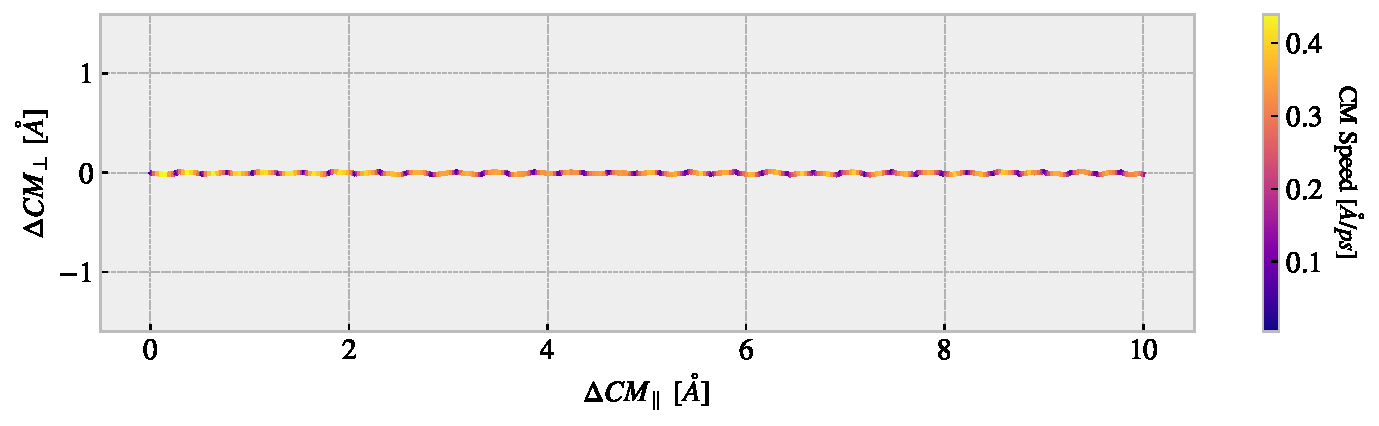
\includegraphics[width=\textwidth]{figures/baseline/COM_path_K0.pdf}
    \caption{Fix move}
    \label{fig:COM_path_K0}
  \end{subfigure}
  \hfill
  \begin{subfigure}[b]{0.85\textwidth}
      \centering
      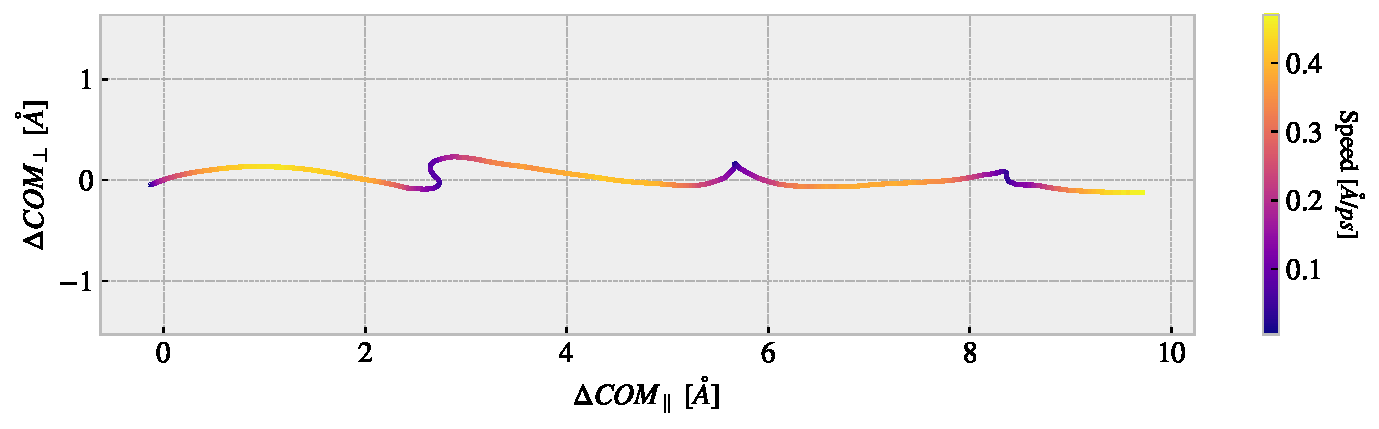
\includegraphics[width=\textwidth]{figures/baseline/COM_path_K30.pdf}
      \caption{K = 30}
      \label{fig:COM_path_K30}
  \end{subfigure}
  \caption{Center of mass relative position from start of drag phase in terms of axis parallel to drag direction $\Delta COM_{\parallel}$ and axis perpendicular to drag direction $\Delta COM_{\perp}$. The colorbar denotes the absolute speed of the COM.}
  \label{fig:COM_path}
\end{figure}




\subsubsection{Defining single metrics with uncertainty}


We are interested in defining single metrics that describe the frictional properties of the sheet. A naturall reference point is the dynamic and static friction coefficient. We can represent these as the mean and max friction force value respectively, but we leave the division by normal force for now as it is only a factor. 


\begin{figure}[H]
  \centering
  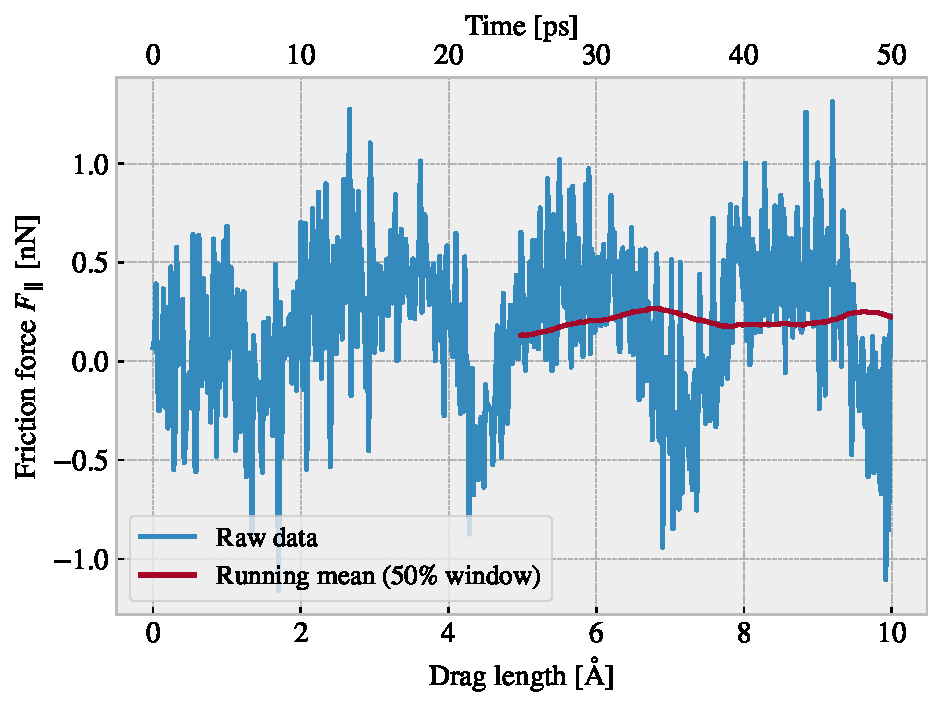
\includegraphics[width=0.7\linewidth]{figures/baseline/Ff_running_mean.pdf}
  \caption{...}
  \label{fig:Ff_runmean}
\end{figure}


A way to quanity the uncertainy of the mean friction evaluation is by looking at the running mean score shown in figure \ref{fig:Ff_runmean}. If the running mean is constant we know that it doesn't really matter whether we stop now to measure or if we drag it a bit longer. However, any fluctuations of this line means that out mean measurement is still sensitive to the drag length. We should not care for flucations in the beginning of the running mean curve as this is essentially including data from the rough beginning transistioning from static to dynamic friction. Only the running mean close to the ending should be considered for our uncertainty. One way is to take then standard deviation in the final 20\% of the running mean curve as a way of approximation the unceetainty of the final mean value. This is shown in figure \ref{fig:Ff_runstd}. 

\begin{figure}[H]
  \centering
  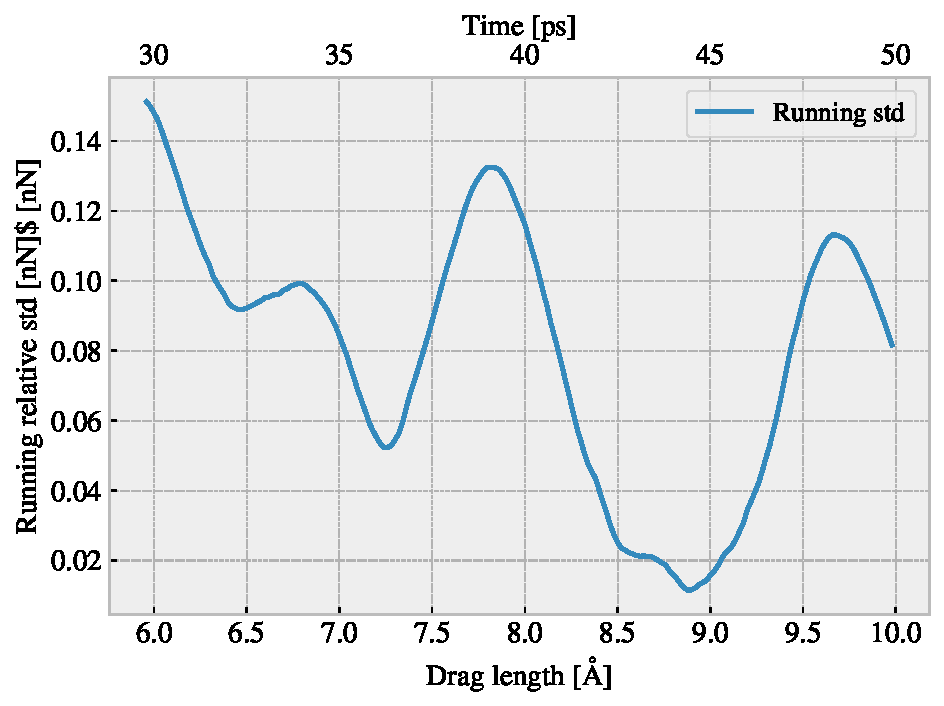
\includegraphics[width=0.7\linewidth]{figures/baseline/Ff_running_std.pdf}
  \caption{Running std (window 20\%) on runmean from figure \ref{fig:Ff_runmean} divided by mean of each window. }
  \label{fig:Ff_runstd}
\end{figure}

From figure \ref{fig:Ff_runstd} we can see that the this provides us with an uncertainty at 8\% relative error when stopping at drag length 10 Å. We also notice that stopping a bit earlier seemed to give better results which reflects the more stable looking part of the running mean roughly between drag length 8 Å and 9 Å. By dragging it for a total of 400 Å we get a final uncertainty of about 3.5 \%. The choice of window size for these running evaluations is somewhat abitrary and thus we should not really trust the exact numric value of the uncertainty, but it serves as an indication of the fluctuations that we are going to pick up in our metrics which we eventually are going to pass on to neural network as true labels. \\

For the max value we do not really have a good way to determine the uncertainty...


\subsubsection{Varying normal force and stretch}

Show multi plot results with uncertainty bars. 


\subsubsection(Varying temperature, drag speed, spring constant and dt)

\begin{figure}[H]
  \centering
  \begin{subfigure}[b]{0.49\textwidth}
      \centering
      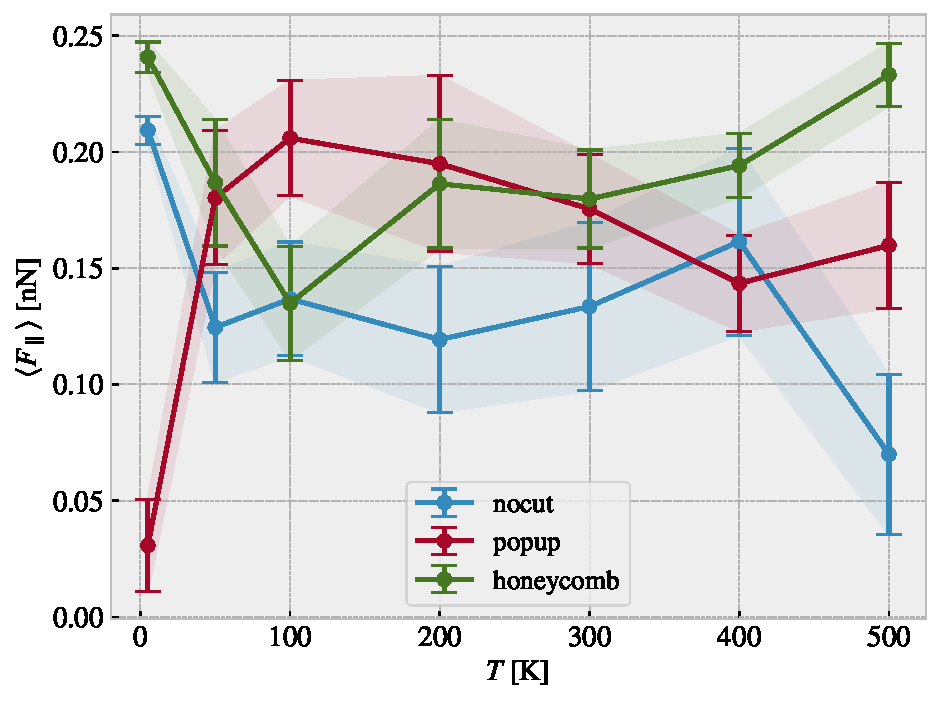
\includegraphics[width=\textwidth]{figures/baseline/variables_temp_mean.pdf}
      \caption{mean friction}
      \label{fig:var_temp_mean}
  \end{subfigure}
  \hfill
  \begin{subfigure}[b]{0.49\textwidth}
      \centering
      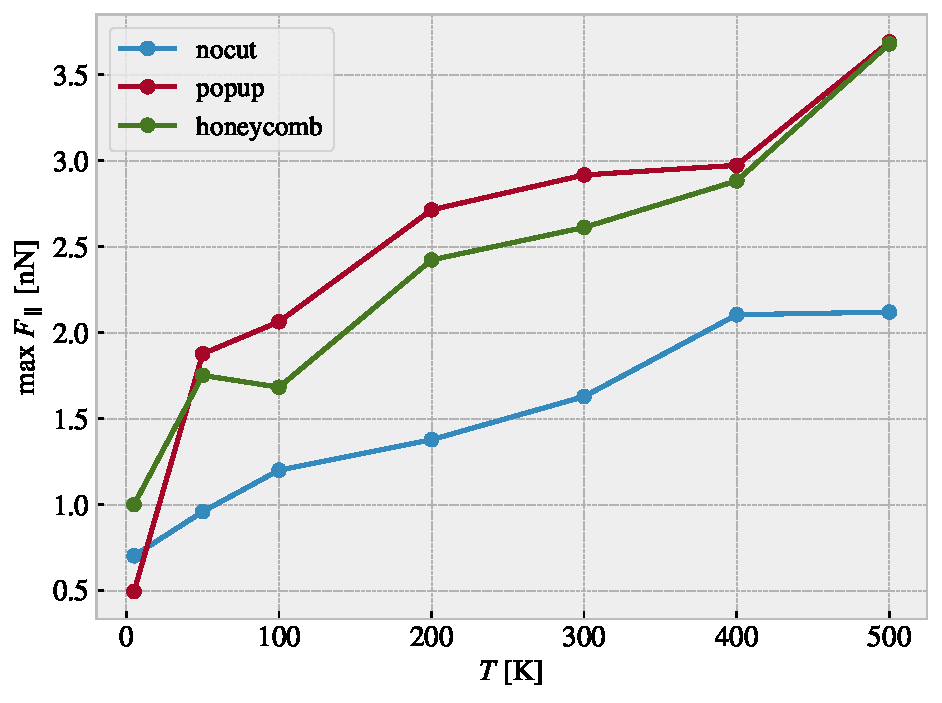
\includegraphics[width=\textwidth]{figures/baseline/variables_temp_max.pdf}
      \caption{max friction}
      \label{fig:var_temp_max}
  \end{subfigure}
  \hfill
     \caption{Temperature}
     \label{fig:var_temp}
\end{figure}

\begin{figure}[H]
  \centering
  \begin{subfigure}[b]{0.49\textwidth}
      \centering
      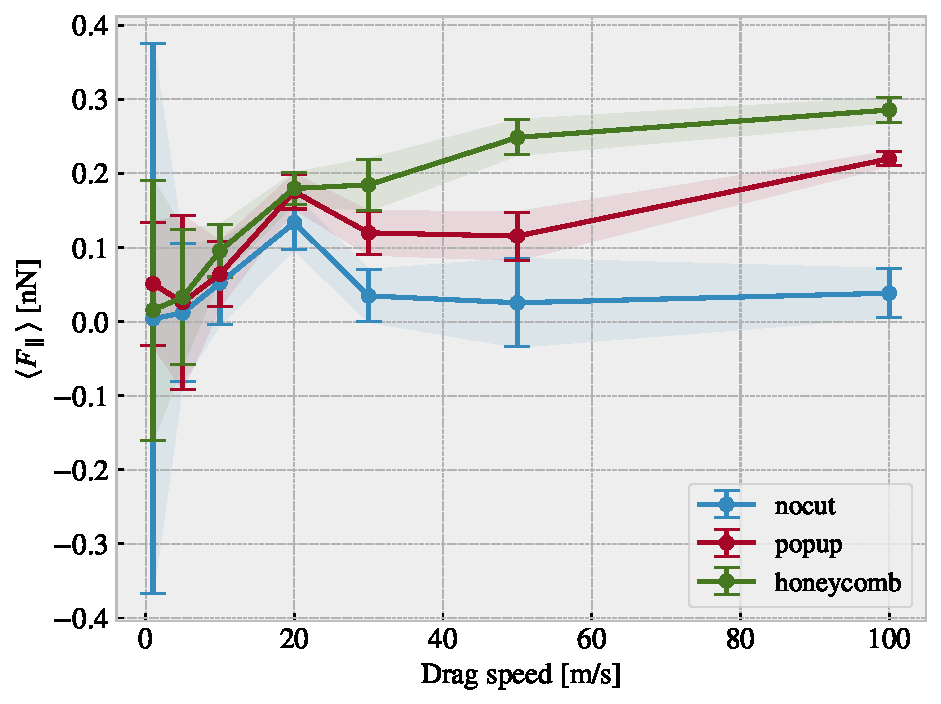
\includegraphics[width=\textwidth]{figures/baseline/variables_vel_mean.pdf}
      \caption{mean friction}
      \label{fig:var_vel_mean}
  \end{subfigure}
  \hfill
  \begin{subfigure}[b]{0.49\textwidth}
      \centering
      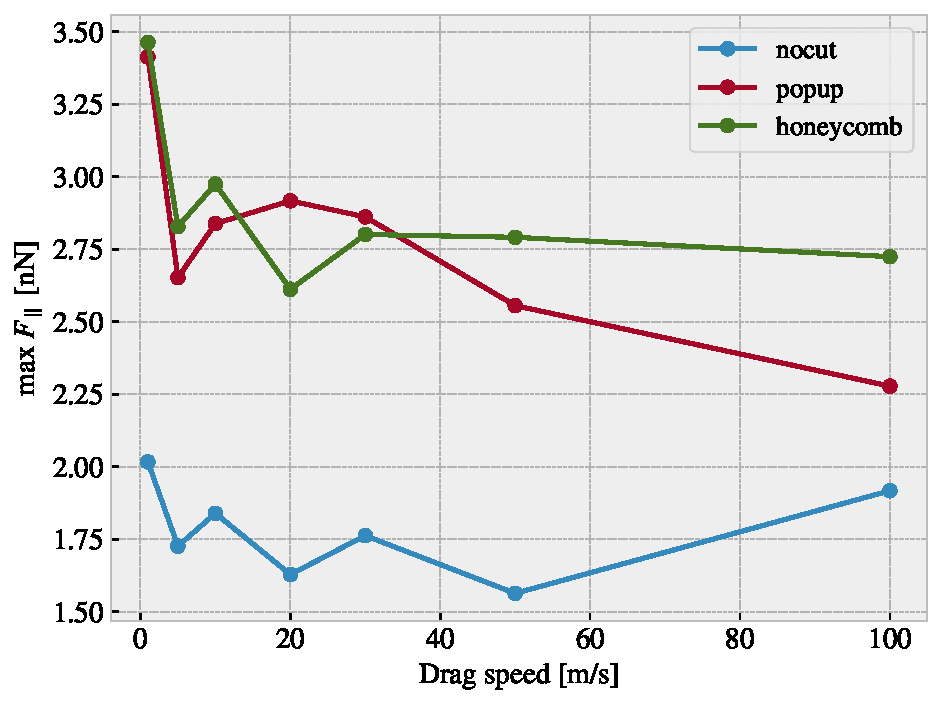
\includegraphics[width=\textwidth]{figures/baseline/variables_vel_max.pdf}
      \caption{max friction}
      \label{fig:var_vel_max}
  \end{subfigure}
  \hfill
     \caption{Drag speed}
     \label{fig:var_vel}
\end{figure}

\begin{figure}[H]
  \centering
  \begin{subfigure}[b]{0.49\textwidth}
      \centering
      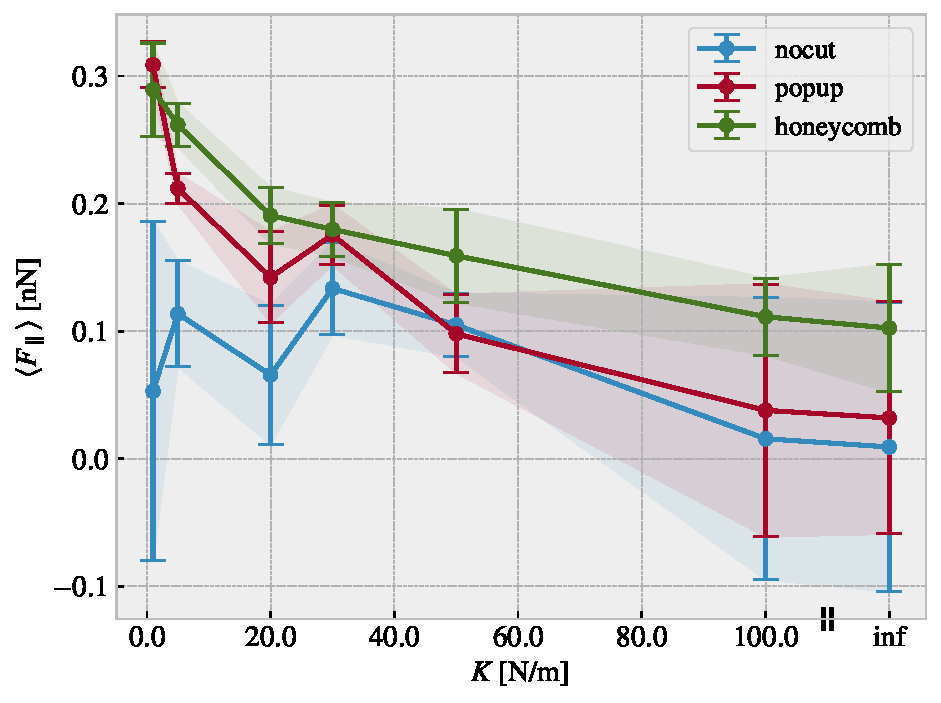
\includegraphics[width=\textwidth]{figures/baseline/variables_spring_mean.pdf}
      \caption{mean friction}
      \label{fig:var_K_mean}
  \end{subfigure}
  \hfill
  \begin{subfigure}[b]{0.49\textwidth}
      \centering
      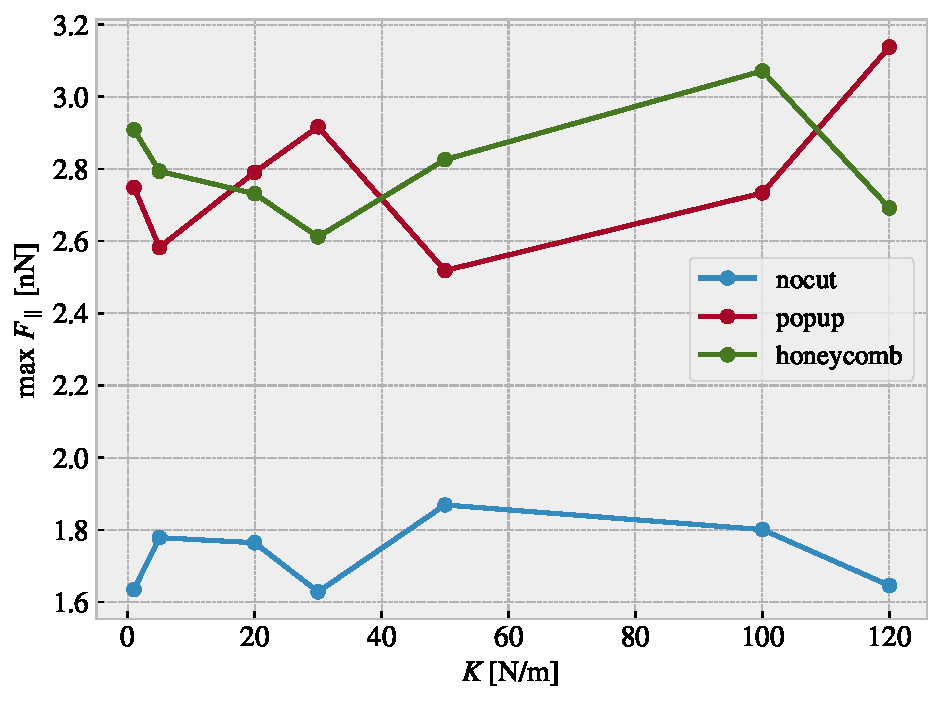
\includegraphics[width=\textwidth]{figures/baseline/variables_spring_max.pdf}
      \caption{max friction}
      \label{fig:var_K_max}
  \end{subfigure}
  \hfill
     \caption{Spring constant}
     \label{fig:var_K}
\end{figure}

\begin{figure}[H]
  \centering
  \begin{subfigure}[b]{0.49\textwidth}
      \centering
      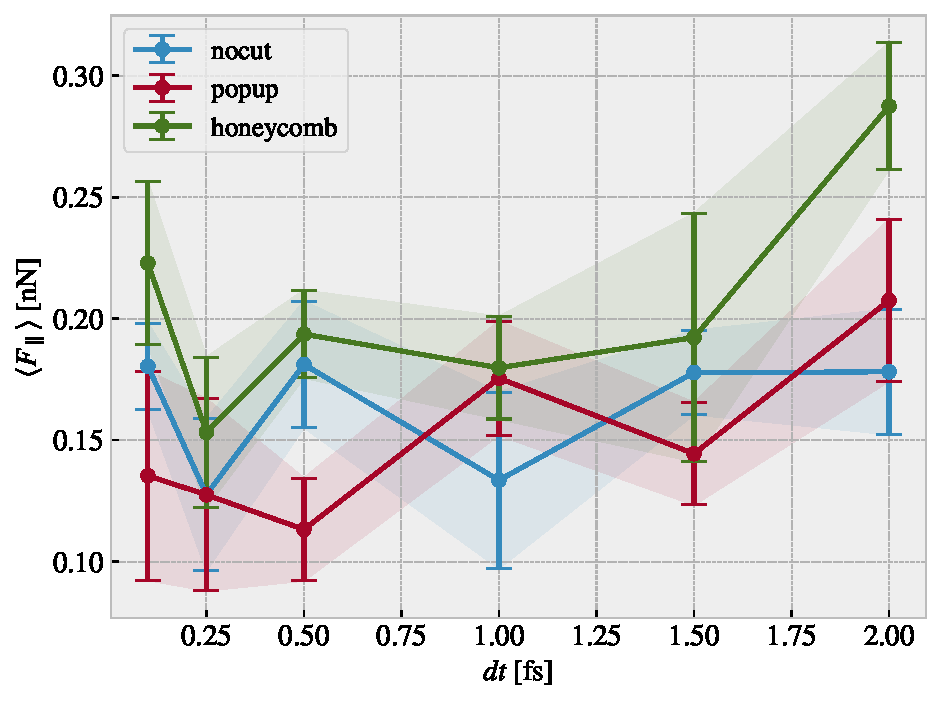
\includegraphics[width=\textwidth]{figures/baseline/variables_dt_mean.pdf}
      \caption{mean friction}
      \label{fig:var_dt_mean}
  \end{subfigure}
  \hfill
  \begin{subfigure}[b]{0.49\textwidth}
      \centering
      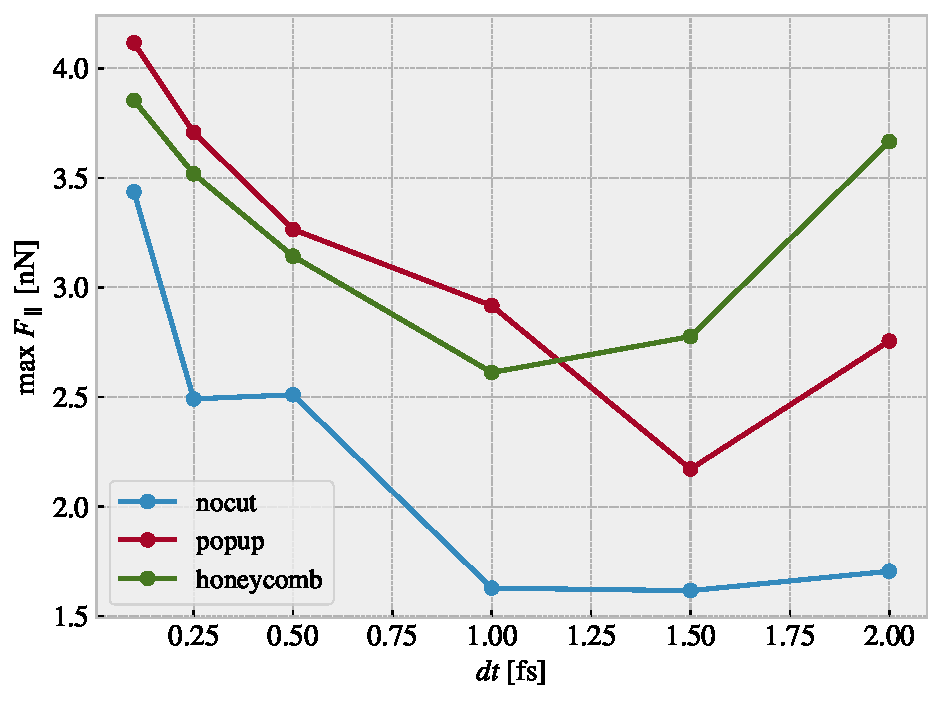
\includegraphics[width=\textwidth]{figures/baseline/variables_dt_max.pdf}
      \caption{max friction}
      \label{fig:var_dt_max}
  \end{subfigure}
  \hfill
     \caption{Timestep}
     \label{fig:var_dt}
\end{figure}

Multi stretch 



\begin{figure}[H]
  \centering
  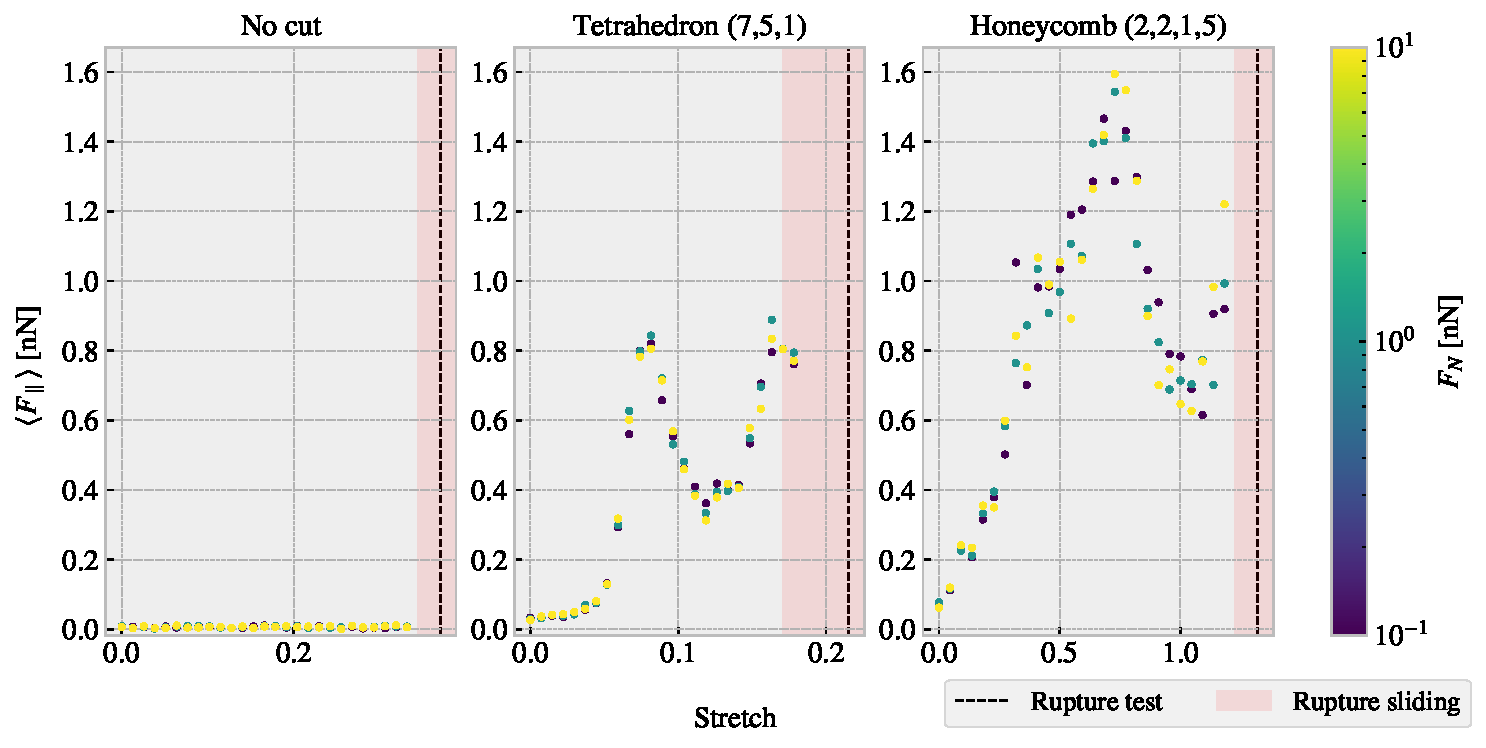
\includegraphics[width=\linewidth]{figures/baseline/multi_stretch_mean_compare.pdf}
  \caption{...}
  \label{fig:}
\end{figure}


\begin{figure}[H]
  \centering
  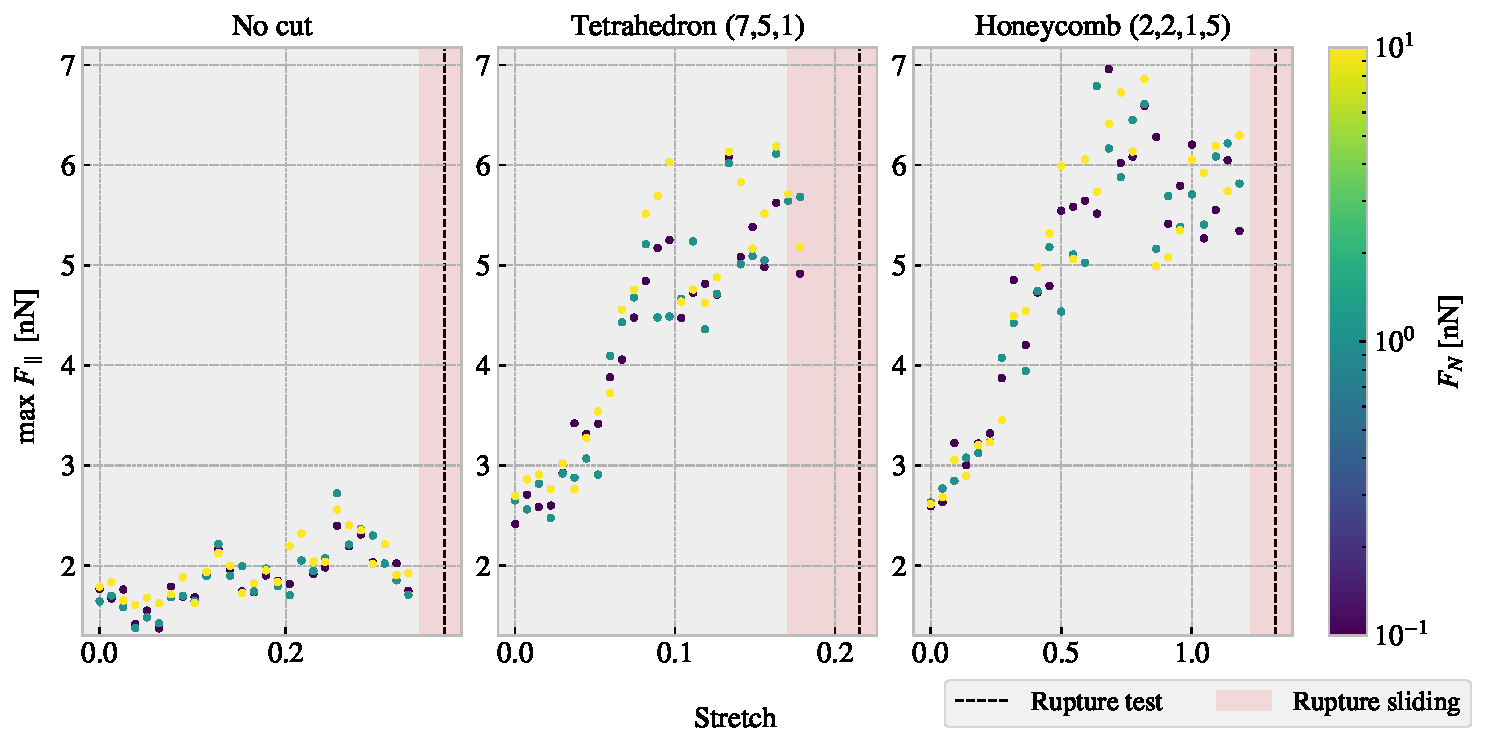
\includegraphics[width=\linewidth]{figures/baseline/multi_stretch_max_compare.pdf}
  \caption{...}
  \label{fig:}
\end{figure}



\newpage
\subsection*{Observations}



\begin{itemize}
  \item stretch $= 0$ \% and $F_N = 188$ eV/Å yielded a very small amount of wear (two atoms visually out of place), for which the sheet dug into the substrate when passing by the second time. For the same normal force but 0.25 \% this problem did not occour. We need to stay out of the friction wear regime. Amorphic substrate is even more prone to this problem of wear.
\end{itemize}